% testando se a classe é lida
%\documentclass{abnt}
%\usepackage[brazil]{babel}  % pt_BR hifenization  
%\usepackage[utf8]{inputenc}  % Allow direct edition with brazilian characters.
%\usepackage[abnt-alf]{abntcite}
%\usepackage{graphicx}

\documentclass[pnumabnt,normaltoc,espacoumemeio,capchap]{abnt}		
\usepackage[brazil]{babel}
\usepackage[utf8]{inputenc}
\usepackage{abnt-alf}
\usepackage{graphicx}
\usepackage{ufc}
\usepackage{multicol}
\usepackage{listings}
\usepackage{eufrak}
\usepackage{subfig}
\usepackage[T1]{fontenc}

% Informações institucionais
\centro{Centro de Ciências}
\departamento{Campus de Quixadá}
\curso{Sistemas de Informação}
\instituicao{Universidade Federal do Ceará}

\tipotrabalho{Monografia}
\autor{Zarathon Lopes Viana}
\autorr{VIANA, Z. L.}
\titulo{Ferramenta de Apoio ao Ensino de Fundamentos de Programação baseada em TDD}
\orientador{Prof. Msc. Camilo C. Almendra} 
\instituicao{Universidade Federal do Ceará}
\local{Quixadá, Ceará}
\cidade{Quixadá}
\data{2012}
\begin{document}
\capa
\folhaderosto

%%% DEDICATORIA %%%
\pretextualchapter{Dedicatória}
	\par Dedico este trabalho a minha família, amigos, e especialmente a minha namorada. Obrigado pela paciência e pela convivência...


%%% Agradecimentos %%%
\pretextualchapter{Agradecimentos}
	\par Aos mestres e a todos que, direta ou indiretamente, contribuíram para a realização deste trabalho.


%%% Epigrafe %%%
\pretextualchapter{Epígrafe}
	\par "Você pode encarar um erro como uma besteira a ser esquecida, ou como um resultado que aponta uma nova direção." \emph{Steve Jobs}


%%% Lista de Figuras %%%
\listadefiguras

%%% SUMARIO %%%
\sumario


%%% INTRODUCAO %%%
\chapter{Introdução}
\par O projeto propõe uma abordagem diferente de ensino de programação para os alunos que estão iniciando em cursos das áreas de tecnologia. Os alunos ao se depararem com as primeiras disciplinas que envolvem programação nas faculdades de tecnologia demonstram um enorme espanto, são várias as frustrações: uma nova linguagem, uma nova forma de raciocinar, o uso das sintaxes das linguagens de programação, as ferramentas de software que na sua maioria são em outro idioma, assim como outras. Como consequência disso, temos altos índices de reprovação nessas disciplinas, muitos alunos, desmotivam-se do curso e até mesmo ocorre evasão por conta dessa frustração de não compreender o que o professor está passando em sala de aula \cite{SI11}.
\par De acordo com os professores que ministram regularmente as disciplinas do ciclo básico, os alunos apresentam um raciocínio lógico mal formado e uma base matemática deficitária, condição que afeta a aprendizagem de fundamentos de programação. Estes professores por outro lado, muitas vezes desmotivam-se ao ver uma turma que não consegue progredir.  
\par A ideia desse projeto é elaborar uma maneira diferente de pensar sobre isso, dando aos alunos mais práticas de programação e aos professores um feedback, quase que imediato, sobre a situação da turma. Sendo assim, os alunos estariam ganhando com relação a estarem exercitando constantemente a programação e os professores estariam avaliando ao mesmo tempo o progresso, ou falhas, dos alunos, podendo propor-lhes em pronto ato, uma nova explicação ou reforço do conteúdo.
\par O principal foco dessa abordagem será a adição de Test Driven Development (TDD), traduzindo ao pé da letra, seria o Desenvolvimento Guiado a Teste. Basicamente consiste em escrever primeiros os testes e depois fazer um programa que faça com que estes teste tenham sucesso. O programador ou aluno consegue com isso atingir dois objetivos: primeiro, ele consegue saber o que está sendo solicitado, segundo, ele terá uma maior compreensão do que está fazendo, desenvolvendo assim o seu raciocínio lógico para resolver problemas computacionais.
\par Nesse trabalho, o projeto ajuda o aluno aprender a sintaxe básica, capaz de confirmar de forma independente, quando completou com sucesso um exercício. Vale lembrar que o aluno irá prosseguir de forma modular a entender a sintaxe e a compreender a solução do problema. "As grandes tarefas" exercícios são muitas vezes difíceis para os alunos por causa de seu tamanho. Muitas linhas de código precisam ser escritas antes de receber qualquer retorno positivo. Isso pode ser frustrante para os alunos iniciantes, e entediante para alunos avançados. A ideia com o uso do TDD é fazer com que o aluno caminhe em passos de bebês (baby steps), faça um pouco, tenha sucesso, se motive e prossiga com o resto da implementação \cite{TF12}.
\par Esse projeto, na sua essência, vem apresentar uma abordagem diferente do ensino de fundamentos de programação, no projeto adaptarei o método de desenvolvimento de software TDD para o ensino. Como consequência dessa abordagem também teremos a elaboração de uma ferramenta para apoiar essa nova forma de ensinar, todas as disciplinas que a utilizarem, no final da disciplina, mostrará a evolução do aluno. Outro ponto bastante relevante a considerar é que a parte conceitual, não será descartada, ou menos valorizada, a ferramenta disponibilizará todo o conteúdo conceitual, dividido por tópicos para que o aluno consulte quando achar necessário.

%%% OBJETIVOS %%%
\chapter{Objetivos}
\section{Objetivo Geral}
\par Apresentar uma abordagem de ensino de fundamentos de programação baseado em TDD, onde o aluno pratica mais e o professor avalia, corrige, e fornece um feedback para o aluno mais rápido.

\section{Objetivos Específicos}
\begin{itemize}
	\item Desenvolvimento da ferramenta de apoio ao ensino de fundamentos de programação (Modelagem e Implementação);
	\item Verificar a aplicabilidade da ferramenta em um curso, afim de refiná-la no final do curso;
	\item Adaptar a aplicação de TDD para o ensino de fundamentos de programação.
\end{itemize}

%%% Revisao Bibliografica %%%
\chapter{Revisão Bibliográfica}
\par A disciplina de fundamentos de programação é um componente curricular para o aluno que ingressa em cursos da área de tecnologia. Em nível de introdução dos fundamentos de programação, faz parte do conteúdo pragmático primeiramente em passar aos alunos uma base necessária para o desenvolvimento da lógica de programação e da representação do raciocínio através de algoritmos nexos e corretos. Essa disciplina é necessária em muitas outras disciplinas que virão pela frente durante sua vida acadêmica na área de tecnologia.
\section{A problemática do ensino de fundamentos de programação}
\par Tais disciplinas, de algoritmos e programação, são aplicadas no início dos cursos da área de tecnologia. Estas disciplinas são consideradas as mais desafiadoras, pois exigem do aluno um esforço mental maior para a resolução de problemas com base lógico-matemática. Infelizmente não há bons resultados quando o aluno se depara com essas disciplinas, dado seu alto grau de esforço e raciocínio, podemos citar o alto número de problemas de aprendizagem, que transcorrem em reprovações, frustrações e desistências \cite{DE08}.
\par Esse problemas enfrentados pelos alunos vem chamando a atenção de educadores da área. Segundo \citeonline{ME01}, existem algumas causas destas dificuldades, dentre as quais as que mais chamam a atenção são:
\begin{itemize}
	\item Elevado nível de abstração envolvido;
	\item Metodologias tradicionais de ensino;
	\item Heterogeneidade com relação aos conhecimentos da turma, tendo assim ritmos diferentes de aprendizado;
	\item Impossibilidade de atendimento individual do aluno. 
\end{itemize}
\par Fatores como estes supracitados podem levar o aluno de fundamentos de programação à necessidade de um acompanhamento, um apoio, uma orientação maior por parte do professor, que nem sempre é possível ser dado pelo professor. Os métodos de ensino tradicionais nem sempre conduzem de forma adequada o aluno. Entre todos os inúmeros motivos que levam os alunos a terem dificuldade e precisar de ajuda, podemos destacar: erro de sintaxe e semântica, dificuldade no enunciado do problema, dificuldade em elaborar algoritmos mentais e incapacidade de verificar os erros de lógica de programação \cite{GM00}.
\subsection{Caracterização de problema}
\par Com esse projeto, pretende-se mostrar uma abordagem diferente para o problema de ensino de fundamentos de programação, visando quebrar o problema em problemas menores e testar o código escrito pelo aluno.
\par Segundo \citeonline{VL09}:
\begin{citacao}
Quando um aprendiz programa o computador, este pode ser visto como uma ferramenta para resolver problemas. Nesse sentido, a relação de um programa exige que o aprendiz processe a informação, transforme-a em conhecimento que, de certa maneira, é explicitado no problema.
\end{citacao}
\par A definição de problema aqui citado refere-se a \citeonline[p.~9]{DT02}: "é qualquer situação que exija o pensar do indivíduo para solucioná-la".
\par Um dos grandes obstáculos, senão o principal, à programação de computadores é pensar na saída, a solução do problema em questão \cite{CB10}.
\par \citeonline{PO95} faz uma relação de quatro etapas que ele julga principais para a resolução de problemas, são elas: compreensão do problema, elaboração de um plano, execução do plano e o retrospecto. Na compreensão do problema, o aluno procura entender o problema, procurar achar elementos que o ajudem a tentar solucioná-lo. Na etapa de elaboração de um plano o aluno volta o seu pensamento agora para como solucionar o problema, qual a estratégia que vou utilizar, é nessa hora que o aluno foca no algoritmo. Na execução do plano é posto em prática tudo o que foi pensado na elaboração, seguindo o algoritmo que o aluno criou ou pensou. Na última etapa, o retrospecto, fornecerá ao aluno o resultado da sua execução, se ele falhou, ele deverá voltar para a fase de elaboração do plano para reavaliar e refletir sobre o que pode ter dado errado.
\par Ainda sobre o retrospecto, \citeonline[p.~10]{PO95} diz: "Se fizerem um retrospecto da rsolução completa, reconsiderando e reexaminando o resultado final e o caminho que o levou até este, eles poderão consolidar seu conhecimento [...]".
\par Essa visão está alinhada com a filosofia do TDD, onde o código escrito pelo aluno vai ser testado, caso não tenha sucesso de imediato, ele voltará a escrever o código procurando o acerto. No momento em que o aluno acerta, este conhecimento adquirido com o erro, o conhecimento do problema e da solução será absorvido de forma prática.
\par No retrospecto, a figura do erro, não é encarada como um fracasso e serve ao aluno para que o mesmo analise onde o erro ocorreu, procurando solucioná-lo de uma maneira diferente da já feita \cite{CB10}.


\section{Roteiros para o ensino de fundamentos de programação}
\par Existem vários roteiros na literatura sobre o ensino de fundamentos de programação, muitos abordam novos conceitos, novas linguagens, mas em sua essência não deixam de lado itens importantes como: variáveis, algoritmos, funções e outros conteúdo básicos que são primordiais para a aprendizagem do aluno de fundamentos de programação.
\par Em \citeonline{FU1} é proposto um interessante roteiro que utiliza jogos como meio de ensino. O roteiro começa abordando os conceitos iniciais de computação (Sintaxe, Semântica, Arquitetura de Computadores, Dispositivos de entrada e saída e etc.), logo após começa a parte de ensino de fundamentos de programação em si, segue a ordem:
\begin{itemize}
\item Controle de Fluxo por Comandos de Seleção;
\item Métodos e Soluções;
\item Dados compostos como vetores;
\item Conceitos sobre Orientação a Objetos;
\end{itemize}
\par Em \citeonline{FU2} temos um aprofundamento maior sobre os algoritmos e os conceitos de computação. Na primeira parte do livro, o autor foca em mostrar o que são Algoritmos e as Ferramentas de Programação, já na segunda parte, ele começa a demonstrar e conceituar a Programação Estruturada que segue da seguinte maneira:
\begin{itemize}
\item Fluxo de Controle I: Estruturas seletivas;
\item Fluxo de Controle II: Estruturas repetitivas;
\item Subprogramas (subalgoritmos): Procedimentos e funções;
\item Estrutura de Dados I: Arrays e Estruturas;
\item As cadeias de caracteres;
\item Arquivos;
\item Ordenação, busca e intercalação;
\item Ordenação, busca e fusão externa (arquivos);
\item Estruturas dinâmicas lineares de dados (pilhas, filas e listas ligadas);
\item Estruturas de dados não-lineares (árvores e grafos);
\item Recursividade;
\end{itemize}
\par E para concluir o roteiro de ensino, sua terceira parte ele aborda os conceitos de Orientação a Objeto.
\par Então nota-se que nesse roteiro, são abordados assuntos bastantes peculiares e de um nível intermediário, que não é o foco de quem ainda está iniciando na prática de fundamentos de programação.
\par Em \citeonline{FU3} o autor traz uma literatura mais leve, bastante agradável com relação ao roteiro. Um fator que chama atenção é que ele dispõe o roteiro de forma simples e objetiva e traz exemplos de código nas linguagens de programação: Pascal, C/C++ e Java, afim de propiciar ao leitor uma melhor maneira de entender o conteúdo. O roteiro de ensino está disposto da seguinte maneira:
\begin{itemize}
\item Conceitos básico (tipos de dados, conceito de variável e formação de identificadores);
\item Estrutura Sequencial;
\item Estrutura Condicional;
\item Estrutura de Repetição;
\item Vetores;
\item Matriz;
\item Sub-rotinas;
\item Manipulação de cadeias de caracteres;
\item Registros;
\item Arquivos.
\end{itemize}
\par É um roteiro bastante interessante e objetivo. O fato de utilizar as três linguagens de programação para exemplificar o conteúdo, dá uma idéia de como fazer para os alunos e guia o aprendizado de forma mais fácil.
\par O roteiro que irá nortear esse projeto é descrito em \citeonline{TF12}, pois enfoca a questão de teste e o ensino de fundamentos de programação. O roteiro está disposto da seguinte maneira:
\begin{itemize}
\item Mostrar como testar programas;
\item Orientação a Objetos (Classes e Polimorfismo);
\item Atribuições e Operações Matemáticas;
\item Estruturas Condicionais e Repetitivas (if-else, switch, for, while, foreach);
\item Manipulação de strings;
\item Exercícios com problemas do dia-a-dia;
\end{itemize}
\par Vale lembrar que como aqui falamos de ensino de fundamentos de programação o conteúdo de \citeonline{TF12} será adaptado para o uso do paradigma procedural.



\section{Teste de Software}
\par 

\par A grande motivação para os testes de software se dá pela grande complexidade de manipular uma grande quantidade de elementos abstratos e seu comportamento. As interações desses elementos muitas vezes geram uma infinidade de resultados/saídas, dentre as quais temos as esperar e as indesejáveis e imprevistas. Por mais experiente que seja o desenvolvedor e por mais esforço que ele tenha na produção e análise dos cenários, é comum surgir erros decorrente das mais diversas interações dos elementos e até mesmo do usuário com o próprio sistema. É necessário, e de certa forma vital, desenvolver testes para dar um feedback pro desenvolvedor do que está acontecendo, o que está ocorrendo com o código produzido em determinados cenário. Esse feedback facilita o aprendizado do desenvolvedor, auxiliar no reparo do código quebrado \cite{TL04}.
\par 
\begin{citacao} 
Portanto, a meta do teste de software é convencer os desenvolvedores e clientes de que o software é bom o suficiente para uso operacional. O teste é um processo voltado a atingir a confiabilidade do software \cite{SV07}.
\end{citacao}
\par Testes de software na sua maioria são apropriados para sistemas de um porte maior, porém sistemas menores também podem fazer uso de testes, porém de forma menos rigorosa. Existem duas principais atividades em testes relacionados a software, são eles de testes de sistema e testes de componentes, ambos feitos por equipes distintas dentro do time de desenvolvimento do software, onde o desenvolvedor de software fica responsável pelos testes de componentes e uma equipe de testes independente fica responsável pelo teste de sistema, vide figura abaixo \cite{SV07}.
\begin{figure}[htbp]
	\centering
	\caption{Fases de Teste\label{fig:f1}. Fonte: Adaptada de \citeonline{SV07}}
	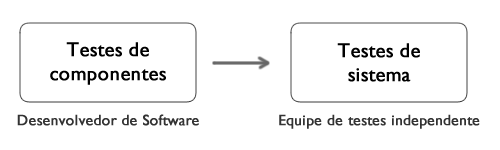
\includegraphics[width=8cm,scale=1]{images/f1.png}
\end{figure}
\par Os objetivos dos testes de componentes é achar, verificar se existem defeitos nos componentes do software, sejam eles funções, objetos, componentes reusáveis. Já o objetivo de testes de sistema está mais focado em descobrir defeitos da integração dos componentes, que são utilizados para formar subsistemas, também é verificado se o sistema atende aos requisitos funcionais e não funcionais para qual foi proposto \cite{SV07}.
\par Em \citeonline{SV07}, existem duas metas distintas sobre o processo de teste de software:
\begin{enumerate}
	\item Demonstrar ao desenvolvedor e ao cliente que o software produzido atende aos requisitos;
	\item Descobrir falhas ou defeitos no software produzido que apresenta comportamento incorreto, não desejável ou em não conformidade com sua especificação.
\end{enumerate}
\par Na primeira meta temos a validação do software, na qual esperamos que o software seja executado corretamente e faça o que se propõe. Na segunda meta expormos os defeitos, os testes são feitos exatamente para o software quebrar e não funcionar. Para o teste de validação, o resultado satisfatório é quando o software funciona corretamente, já para os testes de defeito, o resultado é considerado satisfatório quando o software mostra um defeito causando um funcionamento incorreto no sistema \cite{SV07}.
\par \citeonline{SV07} apresenta um modelo geral de processo de teste de software, vide figura abaixo:
\begin{figure}[htbp]
	\centering
	\caption{Modelo Geral de Processo de Teste de Software\label{fig:f2}. Fonte: \citeonline{SV07}}
	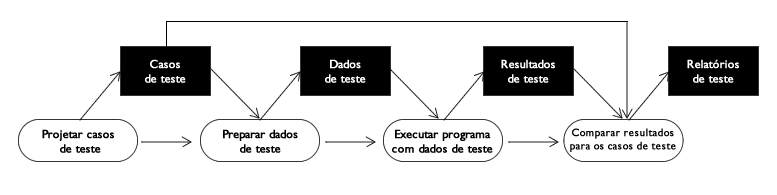
\includegraphics[width=16cm,scale=1]{images/f2.png}
\end{figure}
\par Os casos de teste são diretivas de entradas para o teste e as saídas esperadas, adicionado da descrição do que está sendo testado. Dados de teste são as entradas selecionadas para servir de entrada para os testes, em sua maioria gerados automaticamente através de softwares específicos. Nos resultados dos testes temos se as saídas esperadas foram alcançadas ou não, caso não tenham sido alcançadas, deve-se anotar qual o erro encontrado. No relatório de teste temos a junção de todos os casos de testes, suas entradas, saídas esperadas e saída alcançadas.
\par Geralmente são utilizados dois tipos de testes: teste de unidade e teste de aceitação.
\subsection{Testes de Unidade}
\par Testes de unidade são os escritos pelos desenvolvedores enquanto estes codificam o sistema, ou seja, aquela ideia inicial de deixar os testes para o final do projeto não vale aqui \cite{TL04}.
\par Os teste de unidade devem ser automatizados e todos devem rodar corretamente durante todo o processo de desenvolvimento do software, caso algum teste chegue a falhar, a prioridade da equipe de desenvolvimento passa a ser corrigir o código que está causando o erro. O grande objetivo dos testes de unidade, como Kent Beck falou, é garantir que o código gerado seja o mais limpo possível \cite{TL04}.
\par Uma das maiores vantagens no caso dos testes de unidade é que o desenvolvedor pensa no teste antes da implementação. Ele começa a entender os detalhes e as hipóteses de uso do código a ser produzido. Fazendo isso, o desenvolvedor está fazendo uma análise mais detalhada do problema. Ele deve codificar somente até o teste passar, nem mais, nem menos \cite{TL04}.
\subsection{Testes de Aceitação}
\par Os testes de unidade nos dão a segurança que as classes do nosso software estão funcionando perfeitamente, porém por mais que isso seja fundamental não é suficiente. Um requisito, estória ou funcionalidade pode utilizar mais de uma classe, e frequentemente são utilizadas mais de uma classe. Para isso existe os testes de aceitação, eles procuram simular a interação entre as classes, procuram simular também a interação do usuário com o software. Podemos dizer que o teste de aceitação é um roteiro de como agir e os resultados a esperar das ações desse roteiro \cite{TL04}.
\par Geralmente criada pelo cliente, ou pela equipe de negócio, pois estes conhecem bem a funcionalidade testada, são eles que conhecem e irão estabelecer quais os passos a serem efetuados naquela funcionalidade em questão. A execução dos testes de aceitação deve ser, preferencialmente, de forma automatizada. Sempre que for adicionada uma nova funcionalidade no software, os testes de aceitação devem ser escritos e testados, com isso no final, teremos uma suíte de testes de aceitação juntamente com os testes de unidade \cite{TL04}.
\par Diferente dos testes de unidade, os testes de aceitação não costumam ser executados com 100\% de acerto. Certamente a equipe terá que conviver com um percentual dos teste que não foram executados com sucesso. Geralmente defeitos nos testes de aceitação demoram um pouco mais e exigem mais esforços para serem reparados do que os testes de unidade.

\section{TDD - Desenvolvimento de Software Guiado a Teste}
\par O termo TDD foi apresentado por Kent Beck por volta de 1999, juntamente com termo Extreme Programming (XP) que advém das novas metodologias de desenvolvimento de software, conhecidas como Metodologias Ágeis.
\par O Extreme Programming é um processo de desenvolvimento de software que volta o foco do desenvolvimento para o cliente, através de diversas práticas dentre elas o TDD (Test Driven Development). O foco do XP é entregar um produto com maior valor em um curto espaço de tempo \cite{TL04}.
\par O termo TDD pode ser traduzido como Desenvolvimento de Software Guiado a Testes, o desenvolvedor antes de codificar seu código, ele escreve testes para guia-lo em seu desenvolvimento \cite{TL04}.
\par Segundo Teles (2004): 
\begin{citacao}
	Adotar o desenvolvimento guiado a testes é seguir o caminho da prevenção. O desenvolvedor incorpora alguns hábitos que irão assegurar que o seu software tenha uma probabilidade menor de contrair uma doença.
\end{citacao}
\par O TDD se apresenta em uma forma de ciclo, vide figura abaixo:
\begin{figure}[htbp]
	\centering
	\caption{Ciclo do TDD\label{fig:f3}. Fonte: Adaptada de \citeonline{KB2003}}
	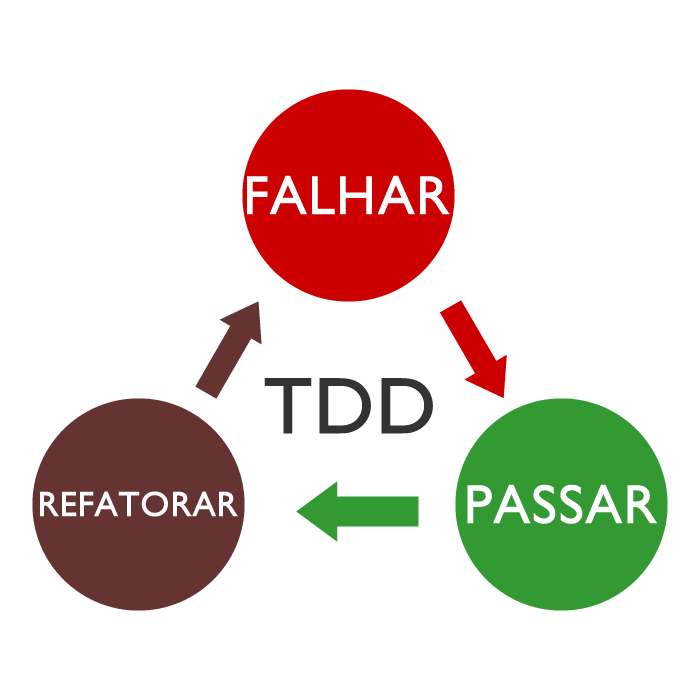
\includegraphics[width=8cm,scale=1]{images/f3.png}
\end{figure}
\begin{itemize}
	\item Na primeira fase, falhar (red), escrevemos um teste, devemos pensar como gostaríamos que a operação aparecesse em forma de código. Em seguida o desenvolvedor executa o teste, certamente ele irá falhar, pois ainda não foi desenvolvido nenhum código, somente o teste;
	\item Na segunda fase, passar (green), o objetivo do desenvolvedor agora é escrever um código que faça aquele teste ter o resultado esperado, ou seja passar, nem que seja de uma maneira rápida, é necessário fazer o teste passar;
	\item Na terceira fase, refatorar (refactor), o desenvolvedor volta para o seu código e o aprimora, utilizando os tipos de dados corretos, alterando as variáveis, enfim, fazendo mudanças que visem melhorar seu código no sentido computacional, em seguida o desenvolvedor refaz o teste.
\end{itemize}
\par O objetivo com isso é que no final o desenvolvedor tenha um código limpo e confiável \cite{KB2003}.


\chapter{Procedimentos Metodológicos}
\par A metodologia proposta para esse trabalho segue as seguintes etapas:
\begin{itemize}
\item Elaboração do conteúdo didático, seguindo a sequência de conteúdos de \citeonline{TF12};
\item Construção da ferramenta de apoio (Análise e Implementação);
\item Aplicação da abordagem proposta em uma turma em forma de curso;
\item Análise dos resultados obtidos no curso. 
\end{itemize}

\par O conteúdo didático do projeto será elaborado de acordo com o roteiro de ensino de programação de \citeonline{TF12}. A linguagem utilizada para o ensino de fundamentos de programação será Ruby, por se tratar de uma linguagem de alto nível, com uma sintaxe bastante amigável e orientada a objetos. O conteúdo irá servir de base para alimentação do sistema de apoio criado e ficará disponível para todos os alunos. A elaboração do conteúdo didático abordará as áreas de testes, fundamentos de programação e uma introdução sobre orientação a objetos (classes e heranças).
\par Ainda com relação ao conteúdo didático, o projeto irá consultar alguns professores que ministram a disciplina de fundamentos de programação no Campus da UFC Quixadá, afim de ajustar os pontos críticos relacionados ao conteúdo.
\par Na fase de construção da ferramenta de apoio, será elaborada uma ferramenta para uso online que irá mostrar todo o conteúdo didático elaborado na fase anterior e disponibilizará os testes para os alunos. Será feita uma documentação do software produzido, mas de forma resumida. A ferramenta vem para complementar e agilizar o processo de entrega de trabalhos e consulta do conteúdo didático. Para o professor, a ferramenta trás ainda uma funcionalidade de verificar como anda o rendimento do aluno, através da análise do seu teste.
\par O projeto foca seus maiores esforços na aplicação da metodologia na prática, em forma de curso com a linguagem Ruby e utilizando a ferramenta que dará apoio a essa metodologia aqui proposta. Serão constituídas duas turmas de 10 alunos, preferencialmente repetentes de fundamentos de programação. A abordagem proposta neste projeto será aplicada em uma das duas turmas, sendo que o conteúdo será o mesmo para as duas turmas. Essa iniciativa será tomada afim de ter uma turma de controle para que na fase de análise possa-se comparar se o uso dessa metodologia foi efetivo ou não.
\par Espera-se ao final do curso fazer um comparativo entre as duas turmas, a de controle e a que utilizou a metodologia. O objetivo dessa comparação é ver se a metodologia mostrou-se mais eficiente que o ensino convencional. O comparativo será nos conteúdos específicos e um comparativo de modo mais geral, abrangendo mais a questão do curso em si. Independente de qual for o resultado, o importante é que os alunos aprendam os fundamentos de programação.

\chapter{Cronograma}
\par Todas as atividades serão realizadas no ano de 2012.
\par
\begin{table}[htbp]
	\centering
\begin{tabular}{lcccccccc}
\hline
Atividade & Mai & Jun & Jul & Ago & Set & Out & Nov & Dez\\

\hline                                                
Elaboração do Conteúdo Didático &  &  & X &  &  &  &  & \\
\hline                                                
Construção da ferramenta de apoio &  &  & X & X &  &  &  & \\
\hline                                                
Aplicação do curso &  &  &  & X & X & X &  & \\
\hline
Análise dos resultados &  &  &  &  &  &  & X & \\
\hline                                                        
Revisão final da monografia &  &  &  &  &  &  & X & \\
\hline                                                       
Defesa do Trabalho Final &  &  &  &  &  &  &  & X\\
\hline
\end{tabular}
\end{table}
\normalsize

\bibliographystyle{abnt-alf}
\bibliography{bib}
\end{document}
